%This is paper.tex

%Write the contents of your paper here.

\newcommand{\degree}{$^\circ$}

\section{Introduction}
Tree volume measurement is one of the many parameters used when documenting and profiling trees and is at the center of forest inventory.Estimates of tree volume are important for planning timber harvests and modelling carbon sequestration. The need for information about Earth's natural resources, including tree volume, has been increasing exponentially in recent times. To be able to accomplish this in forestry, it is a necessity to be able to collect large amounts of data easily and on a regular basis. 

Unfortunately estimating tree volume is expensive, time consuming and in most cases the data collected doesn't meet today's standards \cite{digital imaged based tree measurement for forest inventory}.
Most methods used today to measure individual trees are often done manually with a variety of tools. However the use of these analogue approaches does not come without it's downfalls.

The measurements required for forest inventory can be achieved through a number of methods. One of them is using a so called biltmore stick. A biltmore stick is similar to a normal ruler but has been specially modified for measuring trees. When standing at a certain distance the user can discern the height of the tree by holding the biltmore stick up to their eye and reading the corresponding number. The biltmore stick can also easily be used to measure the \emph{DBH} (Diameter at Breast Height) of the tree. Of course a biltmore stick tries to be as generic as possible so that it can be used on a variety of trees and therefore has no guarantee of providing an accurate result. Other ways of measuring tree volume include using a combination of lasers and inclinometers or by having a person manually climb up the tree and drop a tape measure down to measure the height. Despite these relatively simple ways of measuring they often leave room for error. That’s why a more common way of getting a precise reading is to cut down trees in the area and then physically measuring them. After the relevant data is collected one applies a stem-profile taper equation that is specific to the species of tree measured. These taper functions are based on numerous measurements and have been refined over the years. The main problem with taper functions is that to get an accurate result they need to be callibrated to hundreds of local conditions and are usually custom made for a certain species in a certain area. This again is cost prohibitive and only so much of a forest can be accounted for in the taper function. Even when one manages to create a new taper function, it is still far from perfect as all trees, even from the same species, differ in shape.

SilviaTerra, a high-tech startup company,is willing to change that and have already developed several tools for scanning, analyzing and mapping areas of forestry to give accurate results. This is achieved through computer exactitude combined with statistical analysis. Recently a new project was started, with this research project developing the mathematical back end, to allow users to easily get a correct volume measurement by only using their smart phone.This project aims to solve the problem of obtaining an accurate volume reading of tree, cheaply and non-destructively. This will be done by using a combination of photos taken of the tree, various sensor data from the phone and mathematical computation.

\section{Background}

\begin{figure}[!htb]
	\minipage{0.45\textwidth}
		\centering
  		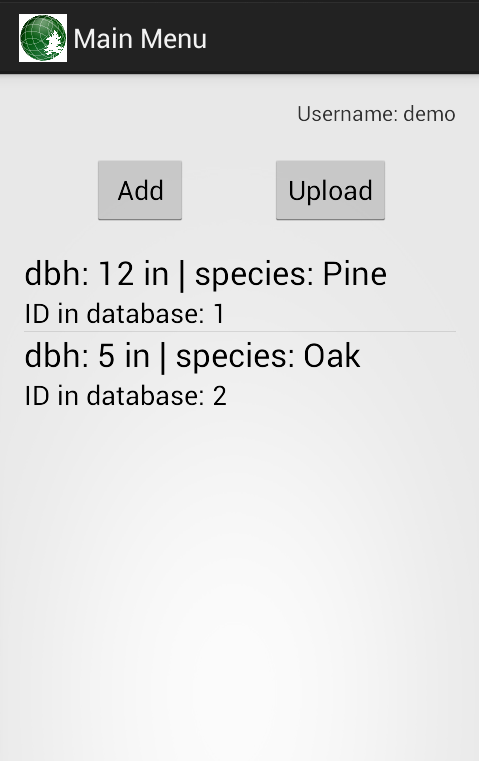
\includegraphics[width=0.65\textwidth]{main.png}
	  	\caption{Homescreen}
  		\label{main}
	\endminipage\hfill
	\minipage{0.45\textwidth}
		\centering
	  	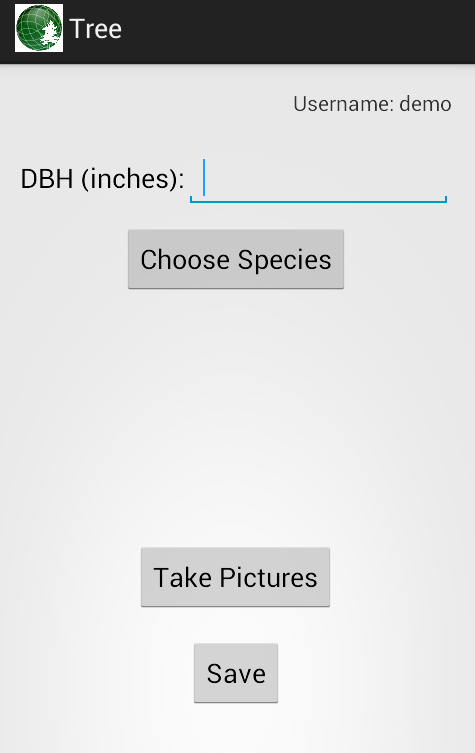
\includegraphics[width=0.65\textwidth]{input.png}
	  	\caption{User input}
  		\label{input}
	\endminipage\hfill
\end{figure}
The first thing a person does when accessing the mobile application is to log into the system with their user name and password. After that they are prompted with a simple menu where they can either choose to add new trees to their inventory or upload them to SilviaTerra's cloud service, figure \ref{main}. The data can then later be used with SilviaTerra's other products. If the user chooses to add a new tree then they will be asked to enter the tree's DBH and species, figure \ref{input}. 
\begin{figure}[!htb]
	\minipage{0.45\textwidth}
		\centering
  		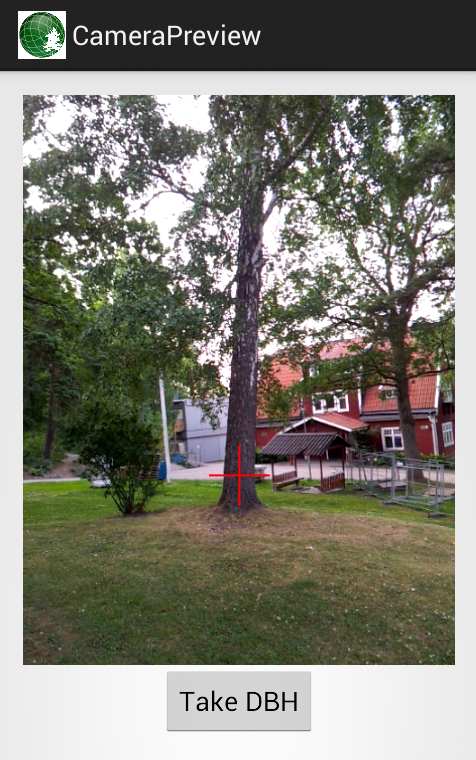
\includegraphics[width=0.75\textwidth]{dbh.png}
	  	\caption{DBH picture}
	  	\label{dbh}
	\endminipage\hfill
	\minipage{0.45\textwidth}
		\centering
	  	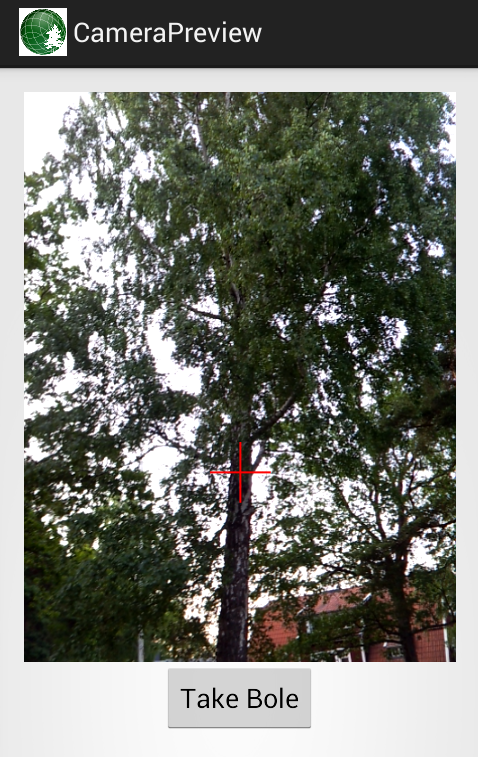
\includegraphics[width=0.75\textwidth]{bole.png}
	  	\caption{Bole picture}
	  	\label{bole}
	\endminipage\hfill
\end{figure}

After that they take two pictures. The interface is quite simple with a cross-hair to show where to point the camera. The first picture is of the actual DBH, figure \ref{dbh}, and the second picture is of the bole of the tree, figure \ref{bole}. Between these two pictures the camera will have to be tilted vertically to capture the bole. The angle between these two camera positions is recorded through the internal gyroscope and accelerometer. After this stage the user's role in the application is done. Now the challenge is to extract useful information from these images. The pictures are sent to one of SilviaTerra's web servers. Here horizontal lines that run parallel with the bottom of the image are drawn across the entire picture. These are drawn at different pixel heights with equal pixel distance in between. The reason this is done is because computer vision is still an experimental technology and is computationally difficult as well as often being error-prone. SilviaTerra has instead opted a different route where the task of edge detection is performed manually by workers at Amazon's Mechanical Turk. So the images with the newly drawn lines are then forwarded to Mechanical Turk. The service in its simplest form a crowd sourcing internet marketplace where individuals or businesses can request tasks to be completed. Usually the tasks are ones that are difficult for computers but easy for humans. SilviaTerra creates tasks where people manually click where the previously drawn lines, cross the edges of the tree. Once the points of intersection are identified, their corresponding pixel coordinates are then paired with the phone sensor data and undergo photogrammetric analysis.

\section{Method}
Once all the required information has been retrieved it is piped into the program that will be calculating the volume. The dataset that is used comprises information about the phone and the results from Mechanical Turk. It is as follows:
\begin{itemize}
	\item DBH length
	\item Horizontal and vertical angle of view
	\item Horizontal and vertical image resolution
	\item Pitch of phone when images are captured
	\item Left and right pixel coordinates from Mechanical Turk
\end{itemize}

\subsection{Distance to tree}
The DBH is used as a reference to find all the other measurements. The first unknown that must be discovered is the distance to the tree. This distance is parallel with the ground. The difference between the x-coordinates of the left and right pixel that correspond to the DBH is calculated, figure \ref{horizontal_triangle}, $X_1$ and $X_2$. Due to the fact that the width of the DBH is now known in both pixels and in a physical measurement (from figure \ref{input} where the user typed it in), the ratio between the two can be determined by dividing the physical distance between $X_1$ and $X_2$ with the number of pixels between them. For example if the width of the tree is 100 pixels and its real life width is 50 centimeters then ratio is 0.5 cm per pixel.
\begin{figure}[htp]
\centering
{
	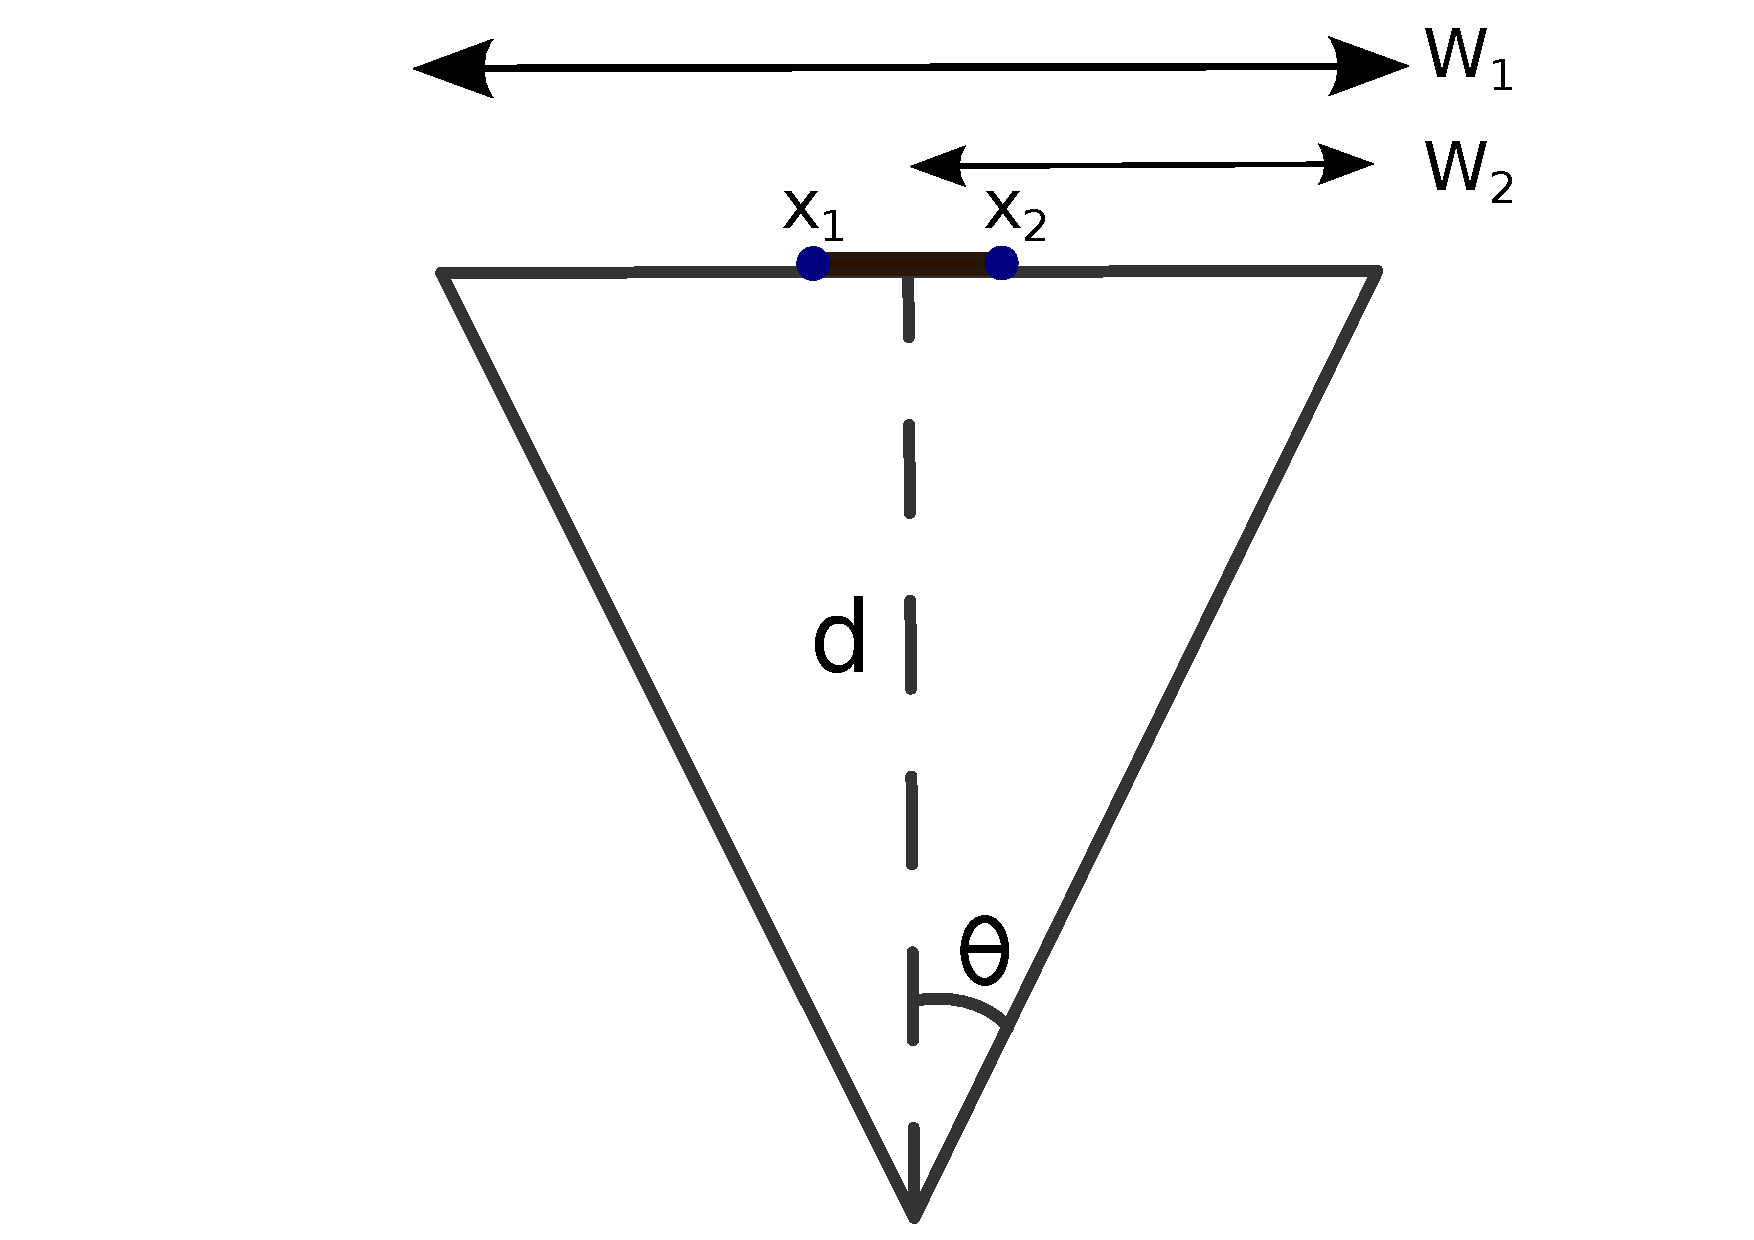
\includegraphics[scale=0.3]{horizontal_triangle.pdf}
	\caption{Birds eye view of horizontal plane}
	\label{horizontal_triangle}
}
\end{figure}
 As seen in figure \ref{horizontal_triangle} an isosceles triangle can be constructed with the horizontal angle of view as the vertex angle. The triangles two congruent legs extend out towards the base of the triangle, $W_1$, which is inline with the tree. To get the length of the base, $W_1$, the previously calculated scale between pixels and the real world is multiplied with the number of pixels in the horizontal resolution of the image. The distance to the tree can easily calculated by drawing an extra line that bisects the vertex angle, resulting in an angle, $\theta$, which is exactly half of the angle of view and the actual distance to the tree $d$. This line also divides $W_1$ into $W_2$ and futhermore produces a right angle triangle that can be solved. Finally to actually calculate the distance, $d$, $W_2$ is divided by $\tan{\theta}$.


\subsection{Heights and widths} 
\begin{figure}[!htb]
	\minipage{0.45\textwidth}
		\centering
  		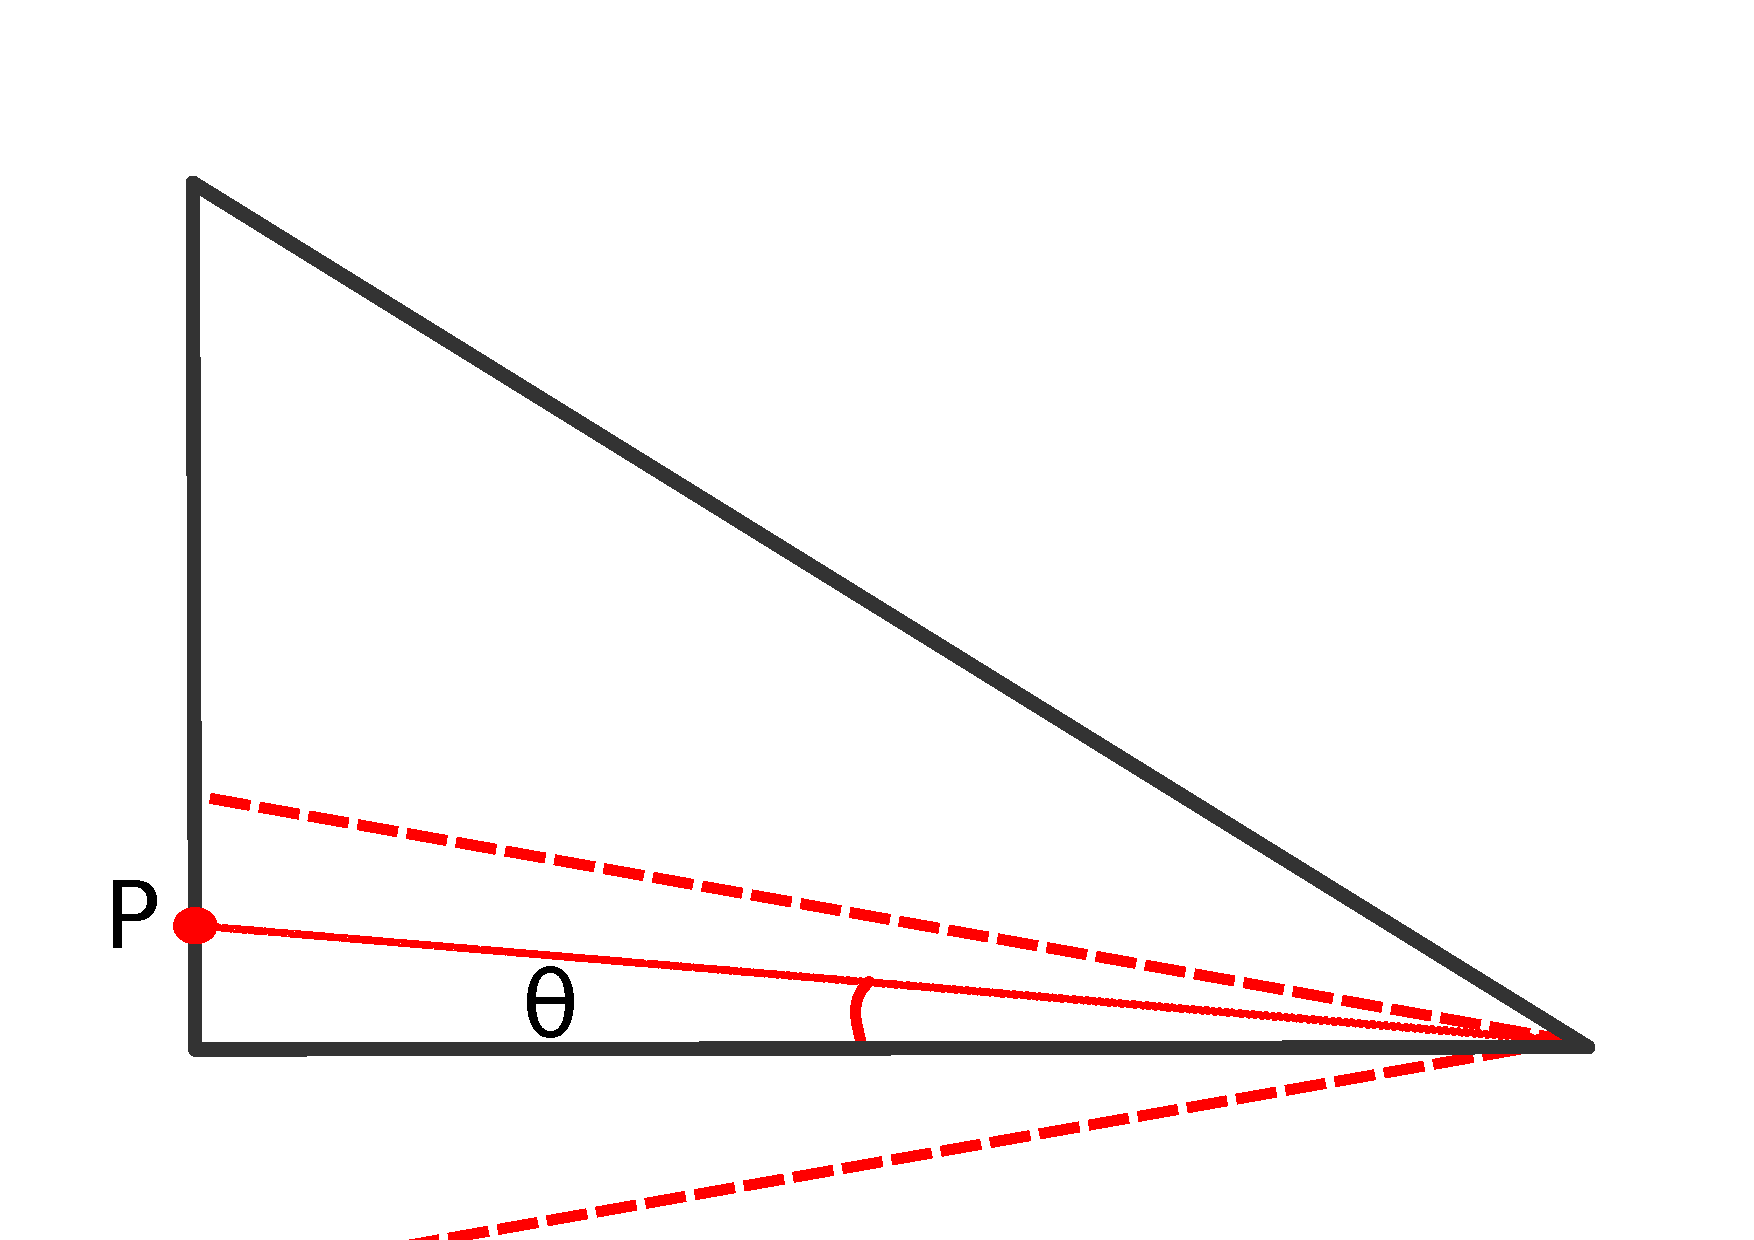
\includegraphics[width=0.9\textwidth]{triangle1.pdf}
	  	\caption{DBH picture}
	  	\label{triangle1}
	\endminipage\hfill
	\minipage{0.45\textwidth}
		\centering
	  	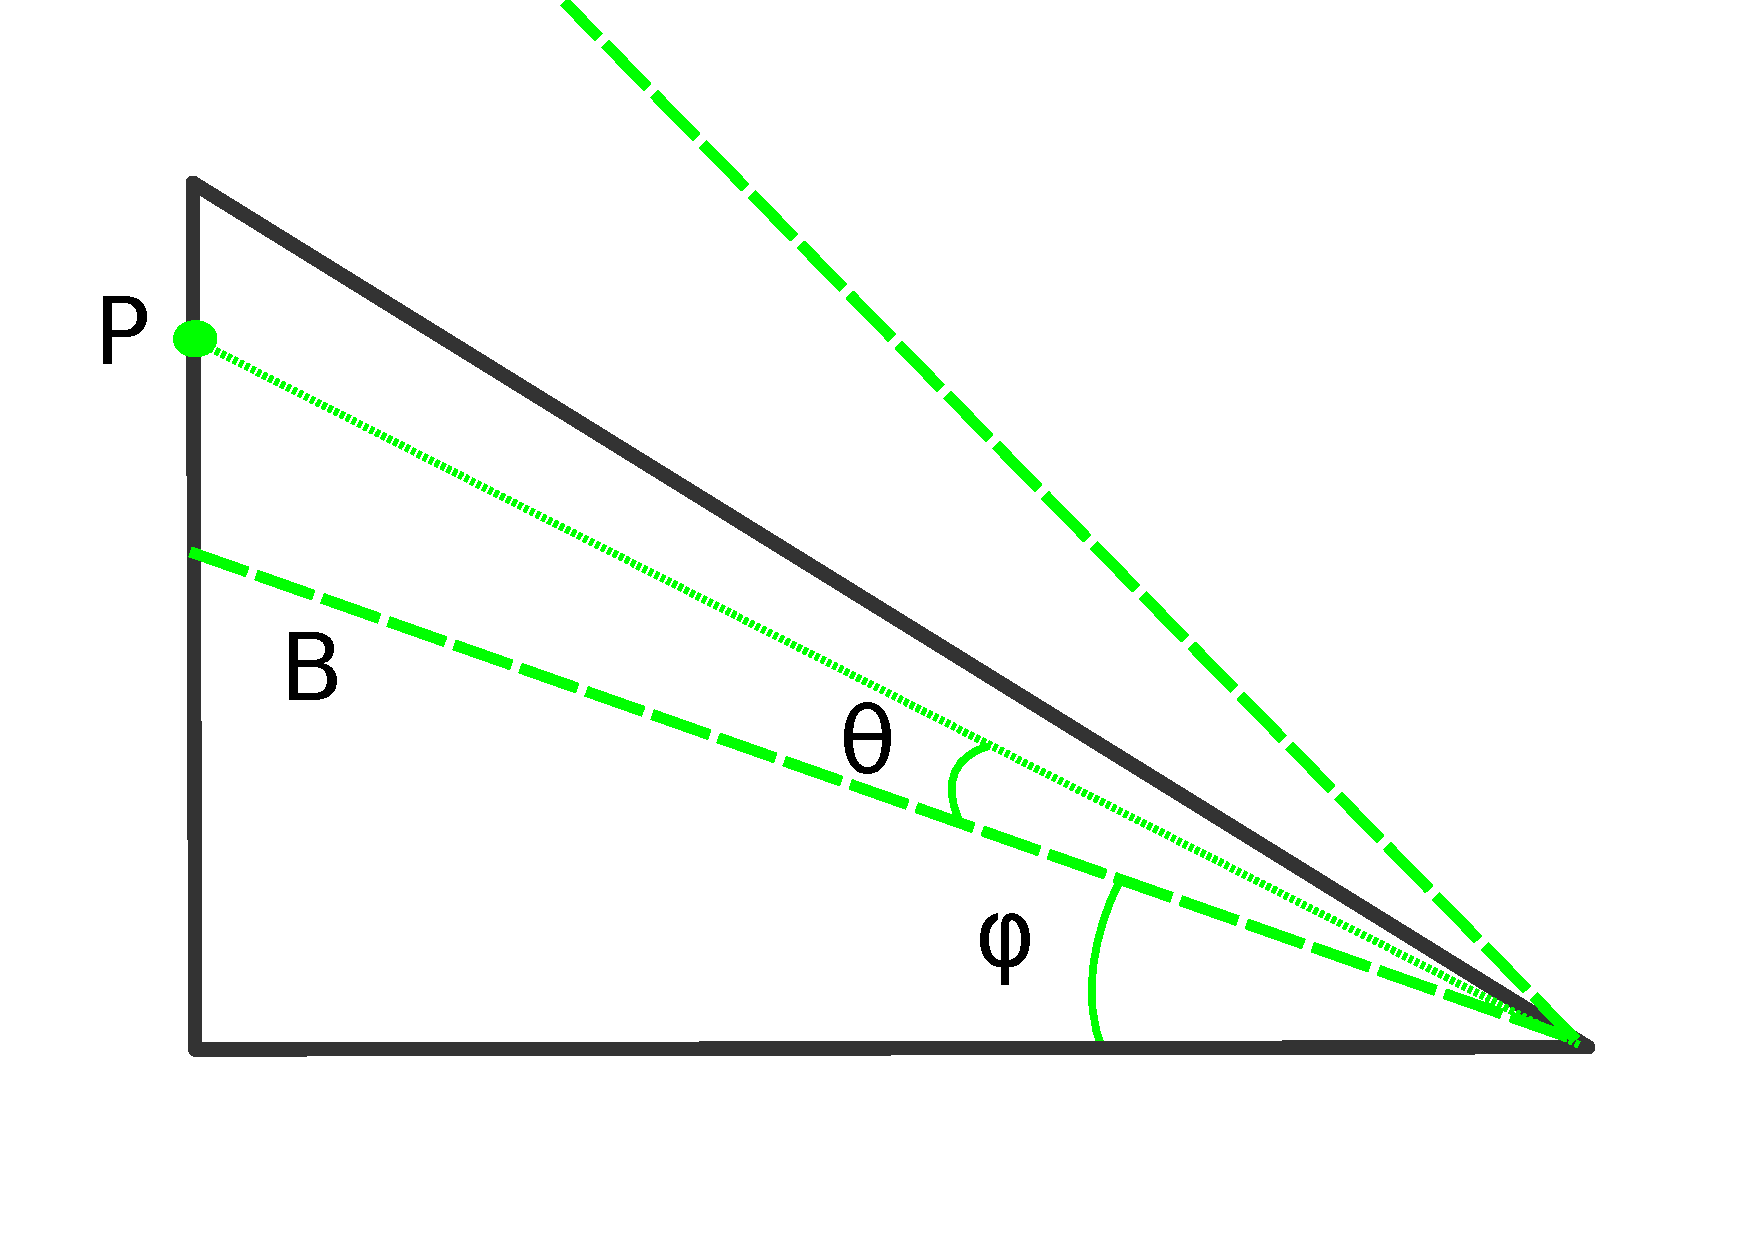
\includegraphics[width=0.9\textwidth]{triangle2.pdf}
	  	\caption{Bole picture}
	  	\label{triangle2}
	\endminipage\hfill
\end{figure}

The next stage is retrieving the real world height to each set of pixel coordinates as well as the width between them, which will be the diameter of the tree. The first step taken is to get the height. The vertical image plate scale, which is the ratio between degrees and pixels in the vertical axis, is calculated by dividing the vertical resolution of the image with the vertical angle of view. For example if the vertical angle of view is 60 degrees and there are 3000 pixels in the vertical resolution then the ratio between the two is 50 pixels per degree. This can be done because it is assumed that the silhouette of the tree is on a plane in the real world which corresponds to the image plane on the camera sensor. Basically the tree doesn't bend towards or from the camera. With this method it is possible to find out the angle to each pixel coordinate, for example $P$ in figure \ref{triangle1} and \ref{triangle2}, in the angle of view. This is angle is denoted by $\theta$ in both figure \ref{triangle1} and \ref{triangle2}. However if the pixel coordinate was identified in the bole image, when the phone was tilted upwards, then angle between the distance to the tree and the lower boundary of the vertical angle of view, $B$, will need to be added, which is represented by $\varphi$ in figure \ref{triangle2}. To calculate the real world height to each set of pixel coordinates, the horizontal distance to the tree, $d$ in figure \ref{horizontal_triangle}, is multiplied wtih the angle to the pixel coordinate. In the DBH picture this angle is just $\theta$ and in the bole picture it is $\theta + \varphi$. The diagonal distance to $P$ is also calculated so that the width can later be determined.

The final part of obataining the parameters for each set of pixel coordinates is to calculate the width between them. This is accomplished by employing the method for calculating the distance to the tree, in reverse. In this case what is known in figure \ref{horizontal_triangle} is the distance $d$, which was the diagonal distance to P, and the angle $\theta$ but not the width of the tree, $X_1$ to $X_2$. $W_2$ is calculated by multiplying $d$ with $\tan{\varphi}$. $W_2$ is then again multiplied by 2, to give $W_1$, and then divided by the number of pixels in the horizontal resolution of the image, once more returning the ratio between pixels and the corresponding real world measurement. To finish off this ratio is the multiplied by the number of pixels between $X_1$ and $X_2$ resulting in the physical width of the tree at that certain height.


\subsection{Volume}
Now the only thing left to produce the final result is to use these newly calculated widths and heights to obtain the total volume. The new calculated heights and lengths are used to calculate a loess curve. A loess curve is a line that is fitted to the input points through local regression. The loess curve is then used to produce a polynomial spline function that can then be used to calculate the diameter at very small height intervals. At each new interval the volume can be calculated and is then added onto the current total volume. This will result in a much more accurate reading than by just numerically intergrating the original points.

This whole process is looped through for every identified pixel coordinate set until the width and height is known for all of them. Once that is done, a new loop is created for calculating the total volume.

\subsection{Simulation}
To test this method a \emph{virtual tree}, that represented a 4m tall tree,was constructed. This tree was made out of blue tape and tapered off drastically so that the program could be thoroughly tested. Along the tape, points were marked out and the height to them plus the width between corresponding points was measured. Just like in the real application, two pictures were taken. One of the DBH and one of the top of the tree. Each set of points was then identified on the pictures and measured in pixels. The parameters were then passed into the program and the results were cross-referenced with the real life measurements.

\newpage

\section{Results}
\begin{table}[h!]
	\begin{center}
		\begin{tabular}{| l c c c c c c r |}		
		\hline
		Measured & 57\degree & 47\degree & 39\degree & 27\degree & 22\degree & 18\degree & 15\degree \\
		\hline
		0 		& 0 	& 0 	& 0 	& 0 	& 0 	& 0 	& 0 	\\
		103 	& 96 	& 100 	& 103 	& 106 	& 113 	& 116 	& 123 	\\
		115 	& 109 	& 113 	& 116 	& 118 	& 125 	& 128 	& 135 	\\
		125 	& 125 	& 129	& 132 	& 134 	& 140 	& 144 	& 150 	\\
		159 	& 142 	& 147 	& 150 	& 151 	& 158 	& 161 	& 167 	\\
		166 	& 158 	& 163 	& 166 	& 167 	& 174 	& 175 	& 183 	\\
		183 	& 173 	& 179 	& 181	& 182 	& 189 	& 192 	& 198 	\\
		\hline
		\end{tabular}
		\caption{Heights over DBH}
		\label{heights}
	\end{center}
\end{table}

\begin{table}[h!]
	\begin{center}
		\begin{tabular}{| l c c c c c c r |}
		\hline
		Measured & 57\degree & 47\degree & 39\degree & 27\degree & 22\degree & 18\degree & 15\degree \\
		\hline
		12       & 11.7      & 12.1      & 12.2      & 12.1      & 12.3      & 12.6      & 11.9      \\
		27       & 26.8      & 28.0      & 28.4      & 28.2      & 28.5      & 28.4      & 28.1      \\
		37       & 36.4      & 37.5      & 38.0      & 37.7      & 38.2      & 38.1      & 37.7      \\
		44       & 42.4      & 43.6      & 44.4      & 44.0      & 44.4      & 44.0      & 44.4      \\
		52       & 51.3      & 52.7      & 53.5      & 53.0      & 53.4      & 52.9      & 53.2      \\
		61       & 60.9      & 62.2      & 63.1      & 62.1      & 62.8      & 62.5      & 61.1      \\
		59       & 59.0      & 59.0      & 59.0      & 59.0      & 59.0      & 59.0      & 59.0      \\
		\hline
		\end{tabular}
		\caption{Widths over DBH}
		\label{widths}
    \end{center}
\end{table}

\begin{table}[h!]
	\begin{center}
    	\begin{tabular}{| l c c c c c c r |}
    	\hline
		Measured & 57\degree & 47\degree & 39\degree & 27\degree & 22\degree & 18\degree & 15\degree \\
		452095   & 418053    & 428738    & 455700    & 451214    & 481471    & 501534    & 492573    \\
		\hline
		\end{tabular}
		\caption{Total volume over DBH}
		\label{volumes}
    \end{center}
\end{table}

\section{Discussion}
\subsection{Error tolerance}
As seen in table \ref{heights} either when the vertical tilt angle is very wide, standing close to the tree, or very narrow, standing far away, leads to error. It's not clear what is causing this but there a two possible reasons. The first one is that because of the short focal length of the camera and overall poor quality when compared to a real camera, causes various forms of distrotion, especially around the edges of the image. When the person is standing close to the tree so the vertical tilt angle is over 45\degree, the points tend to lie exactly there, around the edges of the image. The distortion then affects these points causing the pixel measurements to be incorrect. The other problem occurs in the direct opposite situation, when the person is standing far away and the angle is very narrow. Naturally what happens is that the resolution of the camera just isn't high enough and the pixel measurements just aren't accurate anymore. However most of this distortion seems to only affect the vertical measurements because when looking at table \ref{widths} it is clearly seen that the readings do not stray much at all from their actual values. Despite this the deviation in the height readings still alters the volume calculations, as observed in table \ref{volumes}. Ideally a person should stand so that the vertical tilt angle lies between 45\degree and 25\degree which basically means they should stand somewhere between one tree length to two tree length's from the actual tree.
\subsection{Limitations}
As pointed out in the previous section the main hindrance attatched to this application is the actual camera. The problem is that most mobile phone cameras have a lot of different distortions that make it hard to make accurate measurements. Also when the tree is far away, the resolution of the camera can have a large affect on the final result. Human error is still large factor. If the person is not holding the phone properly, takes a blurry photo or in any other way alters the image, will cause the calculations to be incorrect. Mechanical Turk is also a weak link because it is essentially humans doing the work and there is nothing stopping them from also making mistakes. Although the application has removed a lot of possible human error it has also introduced new machine error. Sensor data from the phone can be inaccurate. The built-in gyroscope and accelerometer can sometimes give very rough measurements and a few degrees can change the whole outcome. Plus if they are not callibrate properly then that will also lead to error.
\subsection{Future development}
The main area that could be expanded on is the edge detection. As explained in the background, today computer vision is still far from perfect. However that will hopefully change in the near future and things like Mechanical Turk can be dropped for a more efficient system that produces little to no error and works autonomously. If camera technology in mobile phones doesn't improve then being able to correct the various distortions would also make an improvement. The possibilty might also exist in the future to have the application calculate extra things like canopy area and volume of external branches and limbs.

